\documentclass[border=4mm,multi=tikzpicture]{standalone}
\usepackage{pgfplots}\pgfplotsset{compat=1.18}
\usepackage{fontspec}\setmainfont{Liberation Sans}
\usepackage{unicode-math}\setmathfont{TeX Gyre DejaVu Math}\newcommand{\Ohm}{Ω}
\usetikzlibrary{arrows.meta,positioning}
\definecolor{dunkel}{HTML}{1F3A5F}\definecolor{heiss}{HTML}{E4572E}
\begin{document}
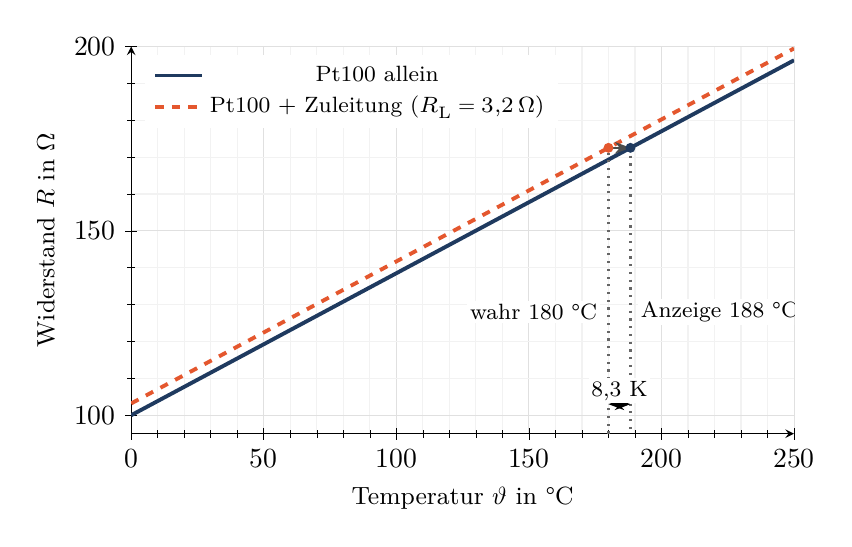
\begin{tikzpicture}
\begin{axis}[width=10cm,height=6.5cm,xmin=0,xmax=250,ymin=95,ymax=200,
  xlabel={Temperatur $\vartheta$ in °C},ylabel={Widerstand $R$ in \Ohm},
  grid=both,grid style={black!12},minor tick num=4,minor grid style={black!5},
  axis lines=left,tick style={black},
  /pgf/number format/use comma,legend style={draw=none,fill=white,font=\footnotesize,at={(0.02,0.98)},anchor=north west},
  every axis label/.style={font=\small}]
\addplot[dunkel,line width=1.4pt,domain=0:250] {100*(1+0.00385*x)}; \addlegendentry{Pt100 allein}
\addplot[heiss,line width=1.4pt,dashed,domain=0:250] {100*(1+0.00385*x)+3.204}; \addlegendentry{Pt100 + Zuleitung ($R_\mathrm{L}=3{,}2$\,\Ohm)}
\draw[black!60,dotted,line width=0.8pt] (axis cs:180,95) -- (axis cs:180,172.504) -- (axis cs:188.3,172.504);\draw[-{Stealth[length=2mm]},black!70,line width=0.6pt] (axis cs:180,172.504) -- (axis cs:188.3,172.504);
\draw[black!60,dotted,line width=0.8pt] (axis cs:188.3,172.504) -- (axis cs:188.3,95);
\fill[heiss] (axis cs:180,172.504) circle (1.8pt); \fill[dunkel] (axis cs:188.3,172.504) circle (1.8pt);
\draw[{Stealth[length=2mm]}-{Stealth[length=2mm]},line width=0.7pt] (axis cs:180,103) -- (axis cs:188.3,103) node[midway,above,font=\footnotesize,fill=white,inner sep=1pt]{8,3 K};
\node[font=\footnotesize,anchor=west,fill=white,inner sep=1pt] at (axis cs:191,128) {Anzeige 188 °C};
\node[font=\footnotesize,anchor=east,fill=white,inner sep=1pt] at (axis cs:177,128) {wahr 180 °C};
\end{axis}
\end{tikzpicture}
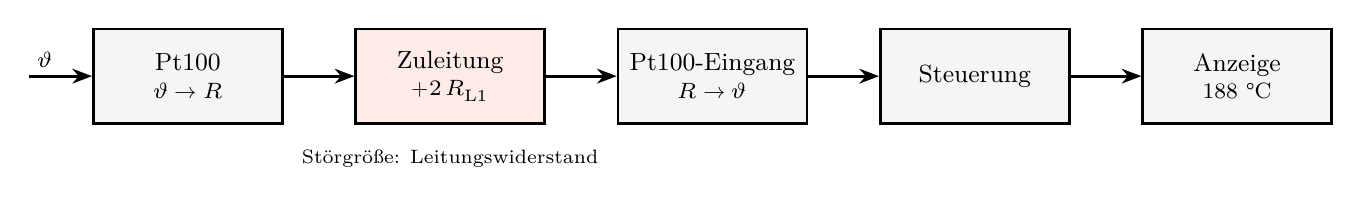
\begin{tikzpicture}[node distance=7mm and 9mm,
  blk/.style={draw,line width=0.9pt,minimum height=12mm,minimum width=24mm,align=center,font=\small,fill=black!4},
  sig/.style={-{Stealth[length=2.5mm]},line width=1pt}]
\node[blk] (s) {Pt100\\[-1pt]\footnotesize $\vartheta \rightarrow R$};
\node[blk,right=of s,fill=heiss!12] (l) {Zuleitung\\[-1pt]\footnotesize $+2\,R_\mathrm{L1}$};
\node[blk,right=of l] (e) {Pt100-Eingang\\[-1pt]\footnotesize $R \rightarrow \vartheta$};
\node[blk,right=of e] (st) {Steuerung};
\node[blk,right=of st] (a) {Anzeige\\[-1pt]\footnotesize 188 °C};
\draw[sig] ([xshift=-8mm]s.west) node[above right=-1pt,font=\footnotesize]{$\vartheta$} -- (s);
\foreach \a/\b in {s/l,l/e,e/st,st/a}{\draw[sig] (\a) -- (\b);}
\node[below=2mm of l,font=\scriptsize,align=center] {Störgröße: Leitungswiderstand};
\end{tikzpicture}
\end{document}
